\section{Risultati con rete SRCNN\cite{dong2014srcnn}}

La fase di training è stata strutturata nel seguente modo:
800 immagini da cui vengono estratte casualmente 20 patch, di grandezza 64x64,
per ogni immagine, ottenendo così circa 16.000 patch per la fase di addestramento.
A differenza del paper SRCNN\cite{dong2014srcnn}
abbiamo scelto di provare a passare i 3 canali RGB come input alla rete invece del canale
di luminanza, ottenendo dei risultati per niente soddisfacenti,
la rete generava un output che presentava parecchi artefatti.

\begin{figure}[ht]
    \centering
    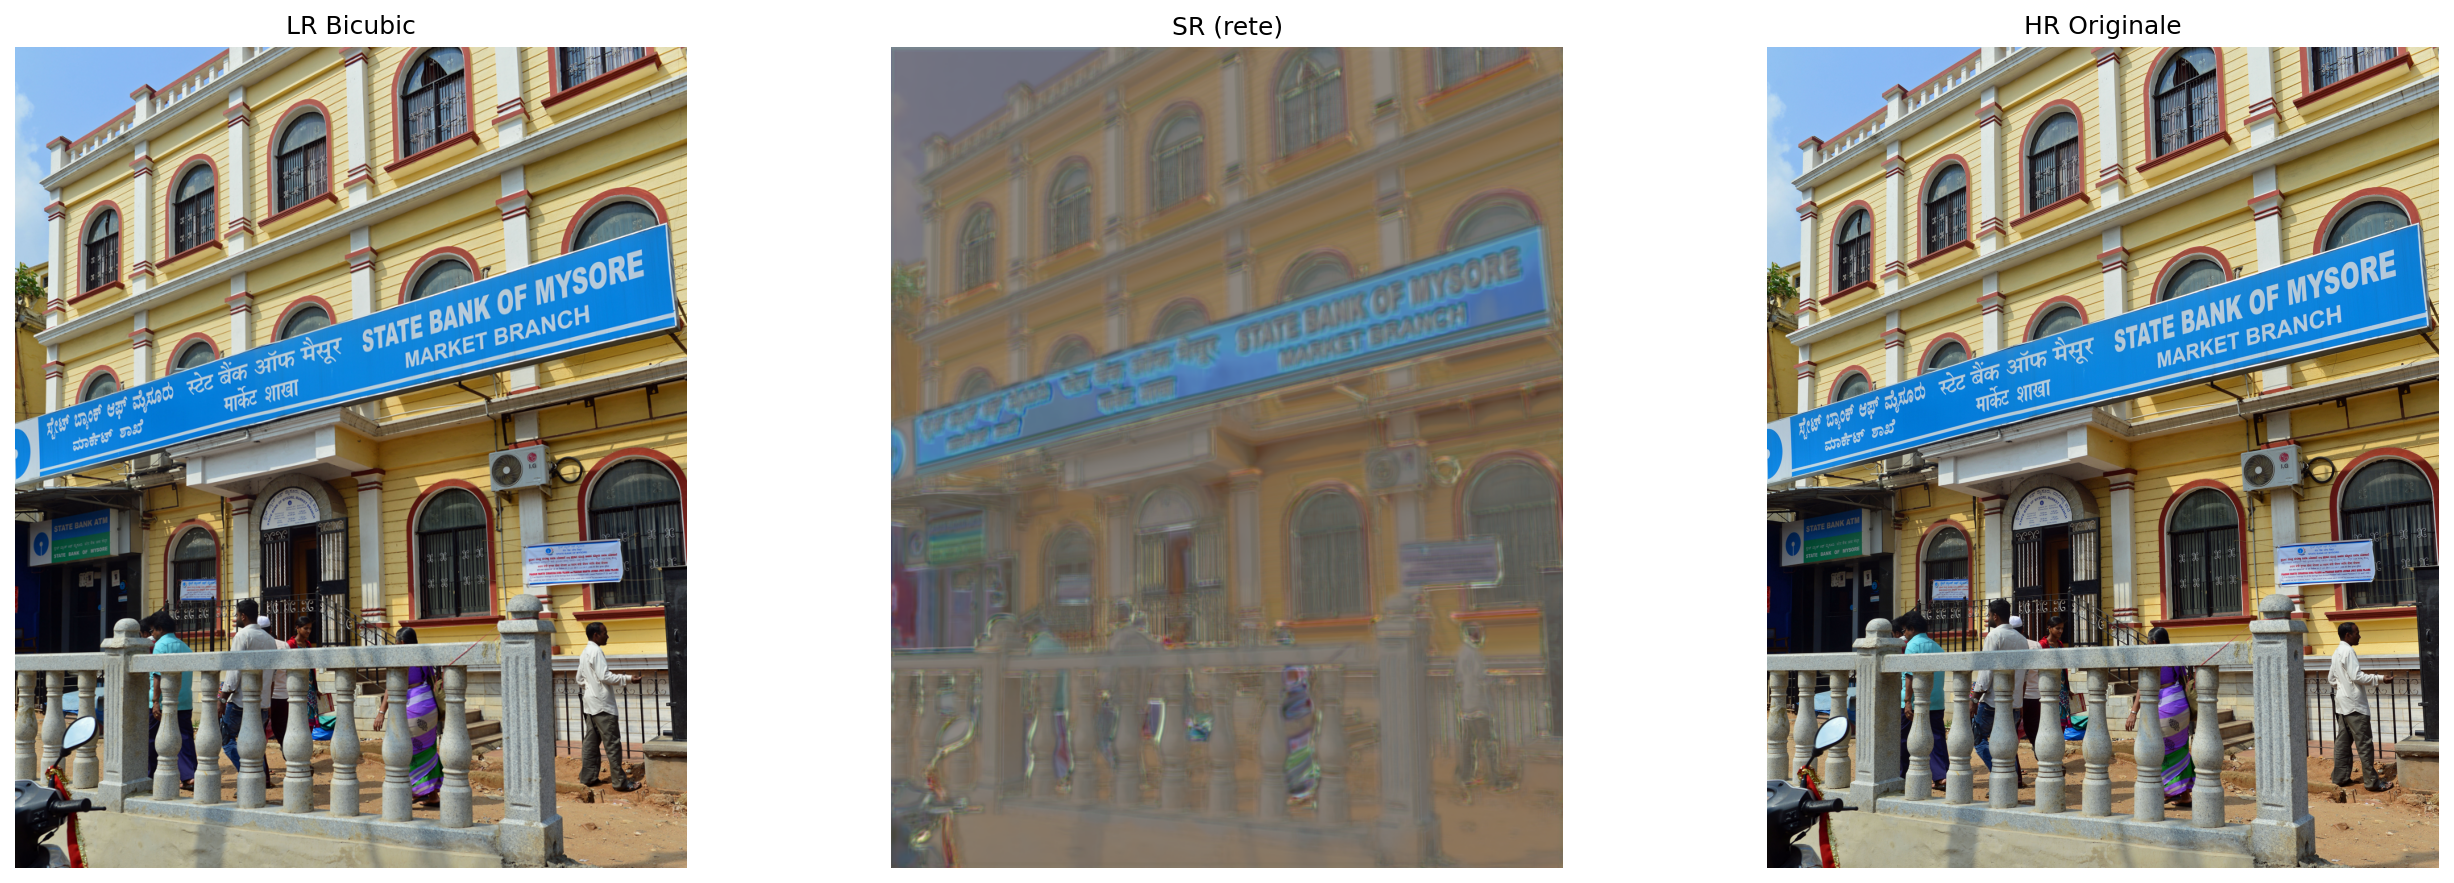
\includegraphics[width=\columnwidth]{figures/confronto_srcnn_150_epochs_2026-05-20_11-07-06.png}
    \caption{Output rete con RGB come input.}
    \label{fig:sr_artefatti_rgb}
\end{figure}

Dopo gli scarsi risultati ottenuti si è deciso di passare solo il canale della luminanza
(Y) alla rete, seguendo quello che è stato fatto nel paper SRCNN\cite{dong2014srcnn}.

Andando a riprodurre l'architettura con 3 layer,
con kernel di grandezza, rispettivamente 9x9, 5x5, 5x5;
con 64 canali in output dal primo layer, con un learning rate di $10^{-4}$ per i
primi 2 layer e per l'ultimo $10^{-5}$.
Abbiamo ottenuto dei risultati migliori rispetto all'approccio RGB,
ma non riuscivamo a superare il PSNR dell'algoritmo di interpolazione Bicubic.

\begin{figure}[ht]
    \centering
    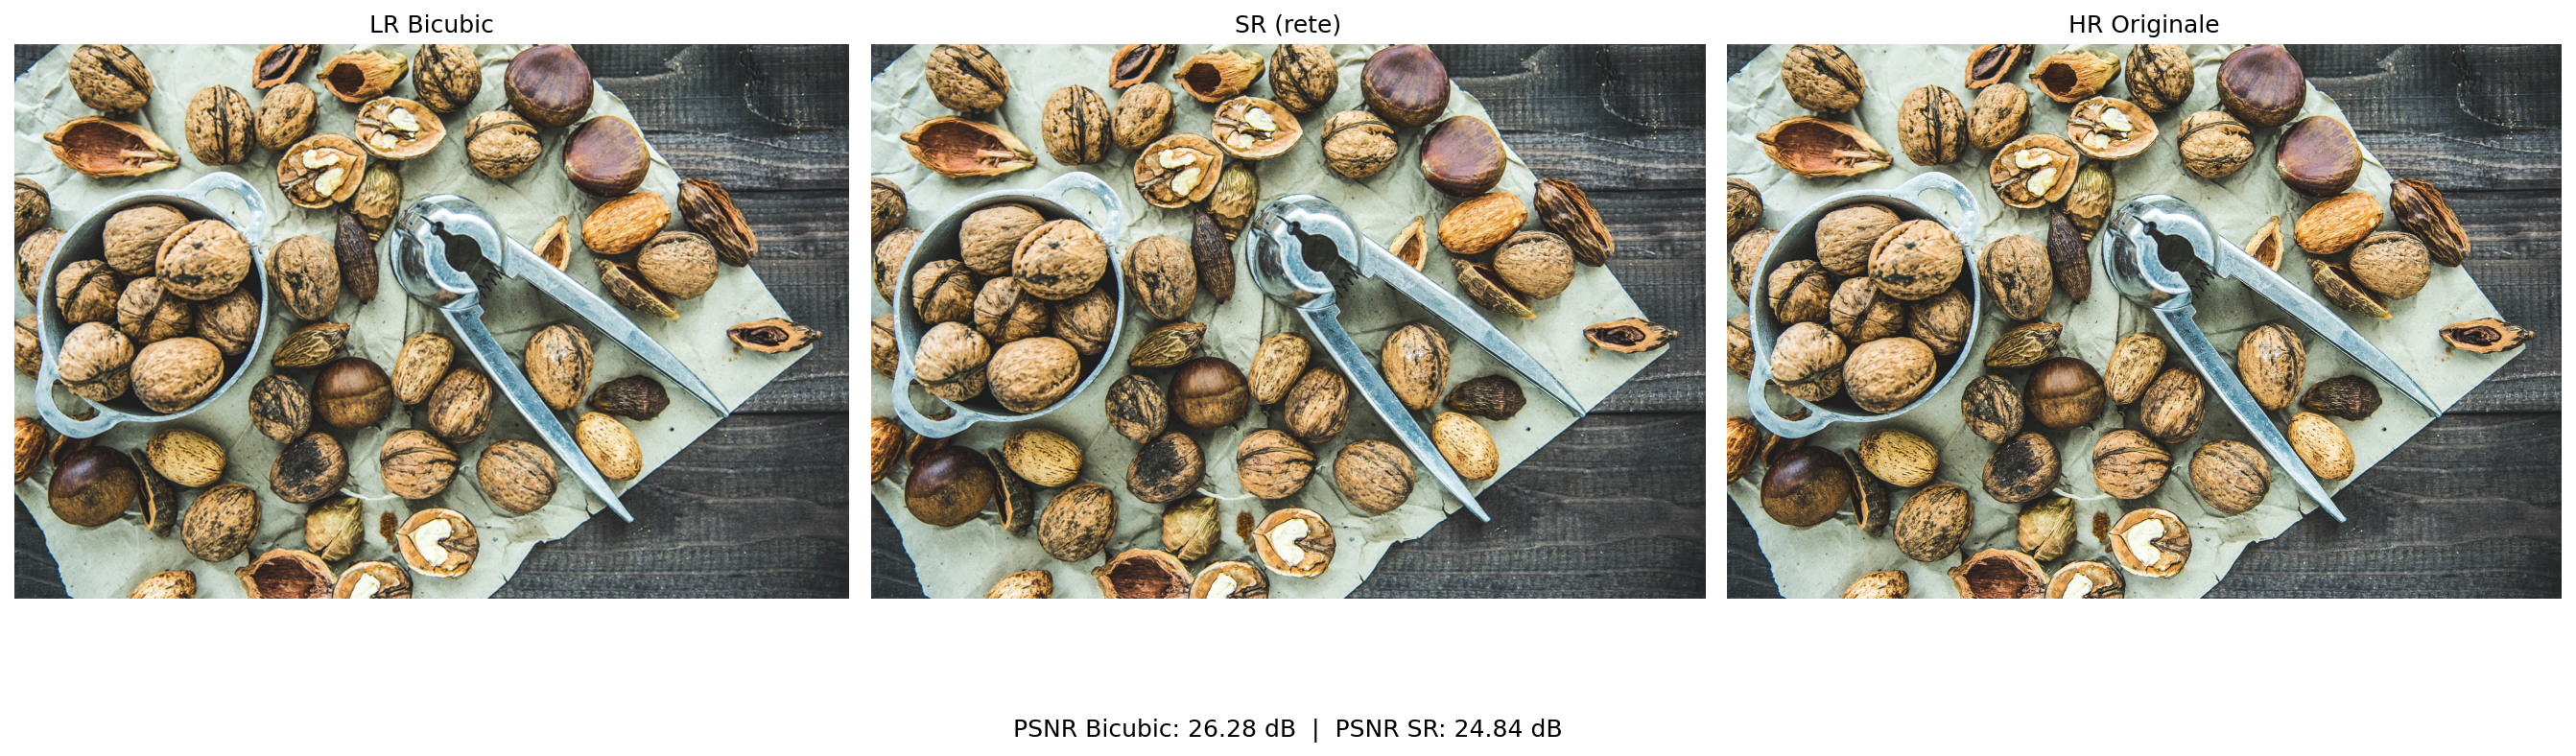
\includegraphics[width=\columnwidth]{figures/confronto_srcnn(9-5-5)_model_600_epochs_2026-05-23_13-06-36.png}
    \caption{Output della rete con input luminanza (Y).
PSNR Bicubic: 26.28 dB, PSNR SR: 24.84 dB}
    \label{fig:sr_Y}
\end{figure}

La fase di validazione è stata fatta estraendo una patch centrale delle
stesse dimensioni delle patch usate per il training, sfruttando il dataset di validation di DIV2K.
In questo modo siamo stati in grado di stabilire come le prestazioni
reali della rete si evolvessero durante la fase di training.

Per la fase di test la rete lavora sull'immagine intera invece delle patch.

Con l'architettura del paper non siamo riusciti a superare bicubic in nessuna istanza del test set,
forse dovuto anche al fatto che abbiamo utilizzato un dataset di training diverso.